\documentclass{article}
\usepackage{tikz}
\usepackage[utf8]{inputenc}
\usepackage{ amssymb }
\usepackage{amsfonts}
\usetikzlibrary{automata,positioning,arrows}

\title{Autómatas y lenguajes formales. Tarea 1}
\author{Fabián Romero Jiménez}
\date{September 6, 2013}
\begin{document}
\maketitle
\begin{enumerate}
\item[\bf{Problema 1}] Las listas de números naturales $L( \mathbb{N} )$ se pueden definir a partir de un elemento básico, la lista vacía
$$ [ ] $$
y la función ::, que toma números naturales y listas y da por resultado nuevas listas. Por ejemplo, si $ n \in \mathbb{N}$ y $[n_{1} . . . n_{m}] \in L(\mathbb{N}) $, entonces $$ n :: [n_{1} . . . n_{m}] = [n n_{1} . . . n_{m}] $$
Considera ahora las funciones $ Sum : L(\mathbb{N}) \rightarrow \mathbb{N} $ y $ doble : L(\mathbb{N}) \rightarrow L(\mathbb{N}) $
$$ Sum([ ]) = 0     $$
$$ Sum(n :: l) = n + Sum(l)   $$
$$ doble([ ]) = [ ] $$
$$ doble(n :: l) = (2  n) :: (doble(l)) $$
Demuestra por inducción que $ 2 \times Sum(l) = Sum(doble(l))$ para toda lista finita l.

\item[Demostración:]
Para el caso de $n = 0$ tenemos que demostrar:
$  2 \times Sum([]) = Sum(doble([]))  $
dado que $ Sum([ ]) = 0  $ tenemos que $  2 \times 0 = Sum(doble([]))  $
y usando que $ doble([ ]) = [ ] $ y tambien que $ Sum([ ]) = 0  $
concluimos que: $  2 \times 0 = Sum([])= 0 $

Con lo que queda concluido el caso base.
Luego, asumamos que es cierto para  $k$
i.e
$$  2 \times Sum(l) = Sum(doble(l)) $$ para toda lista l de longitud $k$
Entonces, sea $l_{k+1}$ una lista cualquiera de longitud $k+1$, por lo que podemos entenderla como $n::l$, donde $n$ el el primer elemento de la lista y l una lista de longitud k, por lo que por hipotesis de inducción tenemos:
$$  2 \times Sum(l) = Sum(doble(l))  $$
y queremos demostrar que:
$$  2 \times Sum(n::l) = Sum(doble(n::l))  $$
desarrollando la parte izquerda tenemos:
$$ 2 \times Sum(n::l) = 2 \times (n + Sum(l))=2 \times n + 2 \times Sum(l) $$
desarrollando la parte derecha tenemos:
$$ Sum(doble(n::l)) = Sum(2 \times n :: doble(l)) = 2 \times n + Sum (doble(l)) $$
y usando la hipotesis de inducción tenemos que:
$$ 2 \times Sum(l) = Sum(doble(l))   \blacksquare$$

\item[\bf{Problema 2}] Dados $0 \le m < k$ y $2 \le p$, sea
$$A_{k,m,p} = \{\alpha \in \{0,1,2,...,p-1\}^\star | x \equiv k (mod\ m) \}$$ donde $\alpha$ es una representación p-aria de x.
Da un método general para construir un autómata que acepte Ak,m,p.

\item[Respuesta]
 Observemos que si tenemos una cadena $c_n$ que es la representación p-aria de un numero $n$ la cadena $c_n$ concatenada del símbolo $x \in \{0,1,2,..,p-1\}$, lo que se hace es equivalente a tomar el número $n \times p + x$ observe que si entonces conocemos la clase a la que pertenece $c_n (mod\ m)$ entonces podemos conocer $c_n \circ x$, pues en el residuo solo importa a la clase a la que pertenece.

Así que el autómata es el sigiente.
\begin{itemize}
\item símbolos $\{0,1,2,..,p-1\}$ que corresponden a la representación p-aria.
\item m estados llamados $\{0,1,..,m-1\}$\\
  Que corresponden a las clases de residuos de m.
\item Estado inicial 0 pues la cadena vacía corresponde al 0
\item Estado final, solamente k, pues nos interesa la clase que es congruente con k (mod m)
\item reglas de producción $\forall r \in \{0,1,2,..,m-1\},\forall n \in \{0,1,2,..,p-1\},  \delta(r,n) = ((r\times p)+n) \% m$ 
\end{itemize}

\item[\bf{Problema 3}] Considera el siguiente autómata no determinista con transiciones-$\epsilon$ .

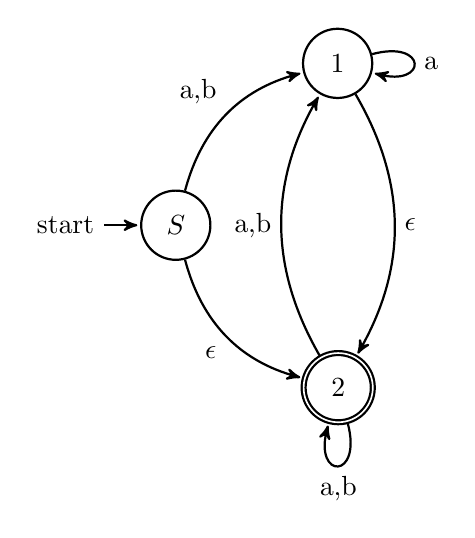
\begin{tikzpicture}[->,>=stealth',shorten >=1pt,auto,node distance=2cm,
  thick,main node/.style={circle,fill=blue!20,draw,font=\sffamily\Large\bfseries}]
   \node[state,initial] (q_0)   {$S$}; 
   \node[state] (q_1) [above right=of q_0] {$1$}; 
   \node[state,accepting] (q_2) [below right=of q_0] {$2$};
    \path[->] 
    (q_0) edge  [bend left] node {a,b} (q_1)
          edge  [bend right] node [swap] {$\epsilon$} (q_2)
    (q_1) edge  [bend left] node  {$\epsilon$} (q_2)
          edge [loop right] node {a} ()
    (q_2) edge  [bend left] node  {a,b} (q_1)
          edge [loop below] node {a,b} ();
\end{tikzpicture}
Transfórmalo en un autómata determinista usando los métodos vistos en clase. Minimiza el
resultado.\\


\item[Respuesta]

\begin{tabular}{ | l || l | l | l  |}
  \hline
    &  $a$    &   $b$  & $\epsilon^\star$ \\
  \hline
$>S$  &  1    &   1  &  S,2 \\    
1   &  1    &   -  &  1,2 \\
(2) &  2    &   2  &  2 \\
  \hline  
\end{tabular}




\begin{tabular}{ | l | l | l |}
  \hline
    &  $a\epsilon^\star$    &   $b\epsilon^\star$  \\
  \hline
$>S$   &  1,2 &   1,2 \\ 
$(1,2)$  &  1,2 &   1,2 \\ 
  \hline  
\end{tabular}


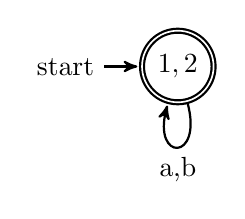
\begin{tikzpicture}[->,>=stealth',shorten >=1pt,auto,node distance=2cm,
  thick,main node/.style={circle,fill=blue!20,draw,font=\sffamily\Large\bfseries}]
   \node[state,initial,accepting] (q_0)   {$1,2$}; 
    \path[->] 
    (q_0) edge [loop below] node {a,b} ();
\end{tikzpicture}

\item[\bf{Problema 4}] Da una expresión regular que genere el lenguaje $\{\alpha \in \{a, b\}^\star | \alpha $ contiene un número par de a o un número impar de b $\}$.

$((aa)^{+}) + (b(bb)^{\star})$

\item[\bf{Problema 5}]Construye un autómata que acepte el lenguaje generado por la expresión $(0+1(01^\star 0)^\star 1)^\star $.
Aplica el algoritmo de minimalización a tu autómata.

Entonces, tenemos los simbolos $010101$ por lo que empezamos poniendo los 6 estados $q_0,q_1,..,q_5$ que corresponen a los símbolos en la expresión y el estado inicial $S$, además por cada simbolo + hacemos una bifurcación y por cada $\star$ una transición $\epsilon$ a donde empieza, así tenemos inicialmente el NFA

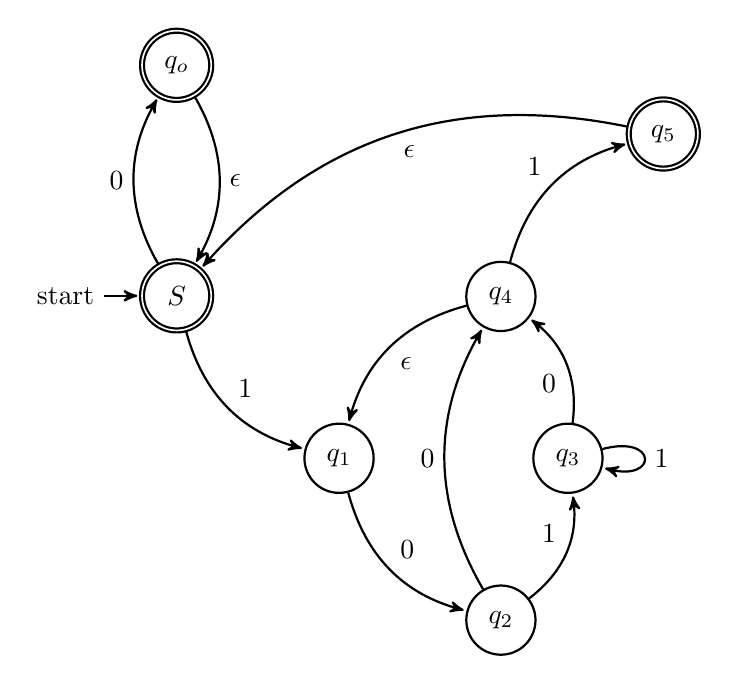
\begin{tikzpicture}[->,>=stealth',shorten >=1pt,auto,node distance=2cm,
  thick,main node/.style={circle,fill=blue!20,draw,font=\sffamily\Large\bfseries}]
   \node[state,initial,accepting] (S)   {$S$};
   \node[state,accepting]         (q_0)  [above=of S]   {$q_o$};
   \node[state ]                  (q_1)  [below right=of S]   {$q_1$};
   \node[state ]                  (q_2)  [below right=of q_1] {$q_2$};
   \node[state ]                  (q_3)  [right=of q_1]       {$q_3$};
   \node[state ]                  (q_4)  [above right=of q_1]   {$q_4$};
   \node[state,accepting]         (q_5)  [above right=of q_4]   {$q_5$};
    \path[->] 
    (S)   edge    [bend left]   node        {0}           (q_0)
          edge    [bend right]  node        {1}           (q_1)
    (q_0) edge    [bend left]   node        {$\epsilon$}  (S)
    (q_1) edge    [bend right]   node       {0}           (q_2)
    (q_2) edge    [bend right]   node       {1}           (q_3)
          edge    [bend left]   node        {0}           (q_4)
    (q_3) edge    [bend right]   node        {0}           (q_4)
          edge    [loop right]   node        {1}           ()
    (q_4) edge    [bend left]   node        {1}           (q_5)
          edge    [bend right]   node        {$\epsilon$}  (q_1)
    (q_5) edge    [bend right]  node         {$\epsilon$}  (S);
\end{tikzpicture}

Y lo transformamos en un DFA

\begin{tabular}{ | l || l | l | l  |}
  \hline
    &  $0$    &   $1$  & $\epsilon^\star$ \\
  \hline
$(>S)$  &  $q_0$   &   $q_1$  &  $S$       \\    
$(q_0)$ &  --      &   -      &  $S,q_0$   \\
$q_1$   &  $q_2$   &   -      &  $q_1$     \\
$q_2$   &  $q_4$   &   $q_3$  &  $q_2$     \\
$q_3$   &  $q_4$   &   $q_3$  &  $q_3$     \\
$q_4$   &  --      &   $q_5$  &  $q_4,q_1$ \\
$(q_5)$ &  --      &   -      &  $q_5,S$   \\
  \hline  
\end{tabular}

\begin{tabular}{ | l || l | l | l  |}
  \hline
    &  $0\epsilon^\star$    &   $1\epsilon^\star$  \\
  \hline
$(>S)$   &   $S,q_0$  &  $q_1$   \\    
$(S,q_0)$&   $S,q_0$  &  $q_1$   \\
$q_1$    &   $q_2$    &  --      \\
$q_2$    &   $q_4,q_1$&  $q_3$   \\
$q_4,q_1$&   $q_2$    &  $q_5,S$ \\
$q_3$    &   $q_4,q_1$&  $q_3$   \\
$(q_5,S)$&   $q_0,S$  &  $q_1$   \\
  \hline  
\end{tabular}

Así tenemos el DFA

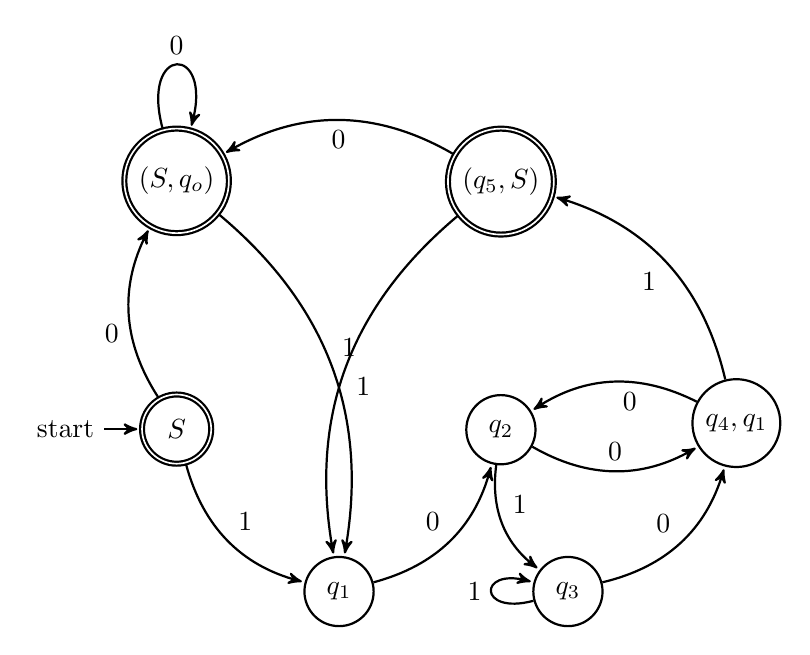
\begin{tikzpicture}[->,>=stealth',shorten >=1pt,auto,node distance=2cm,
  thick,main node/.style={circle,fill=blue!20,draw,font=\sffamily\Large\bfseries}]
   \node[state,initial,accepting] (S)   {$S$};
   \node[state,accepting]         (q_0)  [above=of S]           {$(S,q_o)$};
   \node[state ]                  (q_1)  [below right=of S]     {$q_1$};
   \node[state ]                  (q_2)  [above right=of q_1]   {$q_2$};
   \node[state ]                  (q_3)  [right=of q_1]         {$q_3$};
   \node[state ]                  (q_4)  [above right=of q_3]   {$q_4,q_1$};
   \node[state,accepting]         (q_5)  [above=of q_2]   {$(q_5,S)$};
    \path[->] 
    (S)   edge    [bend left]   node        {0}           (q_0)
          edge    [bend right]  node        {1}           (q_1)
    (q_0) edge    [loop above]   node        {0}           (q_0)
          edge    [bend left]   node        {1}           (q_1)
    (q_1) edge    [bend right]   node       {0}           (q_2)
    (q_2) edge    [bend right]   node       {0}           (q_4)
          edge    [bend right]   node        {1}           (q_3)
    (q_4) edge    [bend right]   node        {0}           (q_2)
          edge    [bend right]   node        {1}           (q_5)
    (q_3) edge    [bend right]   node        {0}           (q_4)
          edge    [loop left]   node        {1}          ()
    (q_5) edge    [bend right]  node         {0}          (q_0)
          edge    [bend right]  node         {1}          (q_1);
\end{tikzpicture}

Minimizando tenemos:
$$ \{q_1,q_2,q_3,(q_4,q_1)\} , \{S,(q_0,s),(q_5,S)\} $$
$$ \{q_1,q_2,q_3\}, \{(q_4,q_1)\} , \{S,(q_0,s),(q_5,S)\} $$
$$ \{q_1,q_3\},\{q_2\}, \{(q_4,q_1)\} , \{S,(q_0,s),(q_5,S)\} $$
$$ \{q_1\}, \{q_3\},\{q_2\}, \{(q_4,q_1)\} , \{S,(q_0,s),(q_5,S)\} $$

y finalmente tenemos el DFA optimizado:

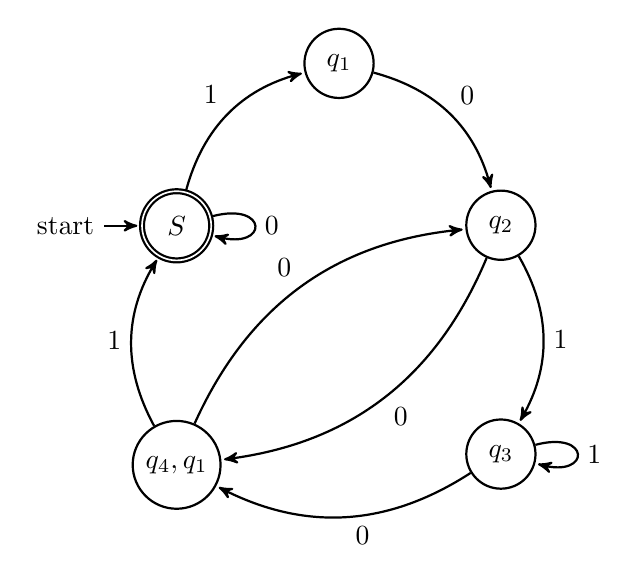
\begin{tikzpicture}[->,>=stealth',shorten >=1pt,auto,node distance=2cm,
  thick,main node/.style={circle,fill=blue!20,draw,font=\sffamily\Large\bfseries}]
   \node[state,initial,accepting] (S)   {$S$};
   \node[state ]                  (q_1)  [above right=of S]     {$q_1$};
   \node[state ]                  (q_2)  [below right=of q_1]   {$q_2$};
   \node[state ]                  (q_3)  [below=of q_2]         {$q_3$};
   \node[state ]                  (q_4)  [below =of S]   {$q_4,q_1$};
    \path[->] 
    (S)   edge    [loop right]   node        {0}          ()
          edge    [bend left]  node        {1}          (q_1)
    (q_1) edge    [bend left]   node       {0}          (q_2)
    (q_2) edge    [bend left]   node       {0}          (q_4)
          edge    [bend left]   node        {1}         (q_3)
    (q_4) edge    [bend left]   node        {0}         (q_2)
          edge    [bend left]   node        {1}         (S)
    (q_3) edge    [bend left]   node        {0}         (q_4)
          edge    [loop right]   node        {1}          ();

\end{tikzpicture}


\item[\bf{Problema 6}]. Demuestra que el lenguaje
$\{\alpha \in \{a, b, c\}^\star | $ la longitud de $\alpha$ es el cuadrado de un natural $\}$
no es regular. Usa el teorema del bombeo.
\item[Respuesta]
consideremos las cadenas $a*$ de longitud $k^2$ 
por el teorema del bombeo tenemos que $\alpha\eta\theta\phi\gamma=a^aa^ea^ta^fa^g$ con $t > 0$ implica que las cadenas $\alpha\eta\theta^i\phi\gamma$ son reconocibles en el lenguaje, pero si $a+e+t+f+g=N^2$, necesitamos que $a+e+2t+f+g=x^2 = k + t$ para alguna $x$, pero tenemos que el proximo cuadrado es $k^2+2k+1$ y $0<t<k$ por lo que $k^2<k^2+s< (k+1)^2$ y contradice a la hipotesis de que está en el lenguage $\blacksquare$

\item[\bf{Problema 7}]. Demuestra que el lenguaje
$\{\alpha \in \{a, b, c\}^\star | \alpha $ es un palindroma $\}$
no es regular. Usa el teorema del bombeo.
\item[Respuesta]
Supongamos que el lenguaje es regular y considere la cadena $a^kbba^k$ que es un palindrome, por el teorema del bombeo tenemos que $\alpha\eta\theta\phi\gamma=a^aa^ea^ta^fbba^k$ es reconocible y por lo tanto $a^aa^ea^2ta^fbba^k = a^{k+t}bba^k$ debe de ser reconocido en el lenguage, pero $a^{k+t}bba^k$ no es palindroma lo cual contradice la hipotesis $\blacksquare$


\item[\bf{Problema 8}]. Resuelve los dos ejercicios anteriores utilizando el teorema de Myhill-Nerode.

\item[Respuesta 6] Para el lenguage que acepta cadenas de longitud $n^2 \forall n \in \mathbb{N}$  Considerese la relación de equivalencia $\alpha \equiv \beta \Leftrightarrow \forall k \alpha a^k \in L \Leftrightarrow \beta a^k \in L$. Entonces $\alpha a^k, \beta a^k \in L  \Leftrightarrow |\alpha|+k =|\beta|+k=n^2, n \in \mathbb{n}$, creando asi una clase de equivalencia por cada $n^2$ que es infinita $\blacksquare$

\end{enumerate}


\end{document}  
